\documentclass[journal]{IEEEtran}
\synctex=0

\usepackage{cite}
\usepackage{amsmath,amssymb,amsfonts}
\usepackage{graphicx}
\usepackage{textcomp}
\usepackage[caption=false,font=footnotesize]{subfig}
\usepackage{booktabs}
\usepackage{url}
\usepackage{xurl}
\usepackage{xcolor}
\usepackage[hidelinks]{hyperref}
\newcommand{\doilink}[1]{\href{https://doi.org/#1}{#1}}
\newif\ifhighlight
\ifdefined\forhighlight\highlighttrue\else\highlightfalse\fi
\newcommand{\rev}[1]{\ifhighlight\textcolor{blue}{#1}\else#1\fi}

\hyphenation{hex-ag-o-nal gran-u-lom-e-try pointy-top}

\begin{document}

\title{Scale Stability of Terrain Opening Spectra on Hexagonal Versus Square Grids}

\author{Yinggang~Guo%
\thanks{Received 23 August 2026; revised 1 November 2026.
This work received no external funding.
(Corresponding author: Yinggang Guo.)}%
\thanks{Yinggang Guo is with the Northwest Institute of Nuclear Technology,
Xi'an 710024, China (e-mail: fariel\_gyg@163.com).}%
}

\markboth{IEEE Geoscience and Remote Sensing Letters,~Vol.~XX, No.~X, Month~2026}%
{Guo: Terrain Opening Spectra on Hexagonal Versus Square Grids}

\maketitle

\begin{abstract}
Square-raster morphological operators are anisotropic: diagonal neighbors lie
a factor of \(\sqrt{2}\) farther than axial ones, so granulometric spectra of
digital elevation models (DEMs) can drift with cell size and with grid azimuth.
Hexagonal cells have a single neighbor distance, yet they have rarely been tested
as a computational basis for terrain pattern spectra.
We compute grey-scale opening spectra on a locally \mbox{equal-area}
\mbox{pointy-top} hexagonal lattice sampled from Copernicus GLO-30 and on the
native square raster,
and we isolate tessellation from structuring-element (SE) area, sampling density,
resampling, and neighborhood.
\rev{Peaks are supplemented by the spectral mean and by Wasserstein-1 (\(W_1\))
distance on the common support \([s_{\mathrm{coarse}},360\,\mathrm{m}]\).
On Yan River loess, whole-window hexagonal \(W_1\) under 30-to-120\,m coarsening
is \(5.2\,\mathrm{m}\) versus \(13.9\,\mathrm{m}\) on the square grid, for
area-weighted or bilinear hex cells. That gap is comparable to area-weighted
lattice-phase noise (\(8.1\,\mathrm{m}\)); nine 30-to-60\,m tiles give median
\(W_1\) \(9.7\,\mathrm{m}\) (IQR \(6.9\,\mathrm{m}\)) versus \(10.8\,\mathrm{m}\)
(\(0.6\,\mathrm{m}\)). The discrete peak ranking does not transfer to a
low-relief Sichuan basin-margin window.
Lattice rotation over \(10^\circ\)--\(60^\circ\) does not give hexagons a
robust advantage: bilinear lattice \(W_1\) is a near-tie, whereas area-weighted
hexagons are \emph{more} rotation-sensitive because they inherit square-pixel
binning.}
Hexagonal tessellation can reduce whole-window coarsening transport of the
opening spectrum on dissected loess, but the practical margin is modest and it
is not a general, rotation-robust substitute for square-grid granulometry.
\end{abstract}

\begin{IEEEkeywords}
Digital elevation models, hexagonal grids, mathematical morphology,
pattern spectrum, scale, tessellation.
\end{IEEEkeywords}

\section{Introduction}

\IEEEPARstart{T}{errain} attributes computed from digital elevation models (DEMs) depend on
the cell size of the raster. Slope, curvature, and contributing area change
systematically as the spatial resolution is coarsened~\cite{zhang1994digital,deng2007dem,evans1972general,wood1996scale},
and elevation error itself is not isotropic~\cite{fisher2006causes}.
Recent global assessments place Copernicus GLO-30 among the most accurate
1$''$ radar DEMs, while confirming that it remains a digital surface
model~\cite{guth2021lidar,simard2024global}.
A second, purely discrete effect is the \emph{tessellation}. On a square lattice the
eight-neighborhood step is anisotropic, so a morphological opening of discrete
radius \(r\) does not mean the same physical half-width in every direction.

Grey-scale granulometry and the pattern spectrum of Maragos~\cite{maragos1989pattern,matheron1975random,serra1982image,soille2004morphological}
summarize how much landform volume is removed as the opening radius grows.
The same idea underpins morphological profiles in high-resolution remote
sensing~\cite{pesaresi2001new,dallamura2010morphological,ghamisi2015survey} and
geomorphological morphology~\cite{sagar2013mathematical}.
Related scale-space and orientation tools in geomorphometry include
multiscale land-surface parameterization and topographic
openness~\cite{wood1996scale,schmidt2003comparison,yokoyama2002openness}.
Almost all of that work is executed on square rasters.

Hexagonal sampling has a single first-neighbor distance and a more
nearly circular discrete disk~\cite{mersereau1979processing,middleton2005hexagonal}.
Equal-area hexagonal discrete global grids are now standard
for global geospatial indexing~\cite{sahr2003geodesic,snyder1992equal}, and
hexagonal lattices have been used for valley extraction, watershed
delineation, and multi-resolution terrain analysis~\cite{wang2020isotropic,liao2020watershed,li2022multi}.
They have not, however, been used as the native domain of a terrain opening
spectrum together with a like-for-like square-grid control, a metric
alignment of the radius axis, and tests that isolate tessellation from
SE size, sampling density, resampling, and neighborhood.

This letter asks: after aligning spectra in meters, does a hexagonal opening
spectrum of a real DEM drift less than the square-grid spectrum when the cell
size is coarsened from 30 to 120\,m and when the sampling lattice is rotated?
We answer it on Copernicus GLO-30~\cite{copernicus2021dem} over a loess-gully
box on the Yan River and a low-relief confirmation box on the western margin of
the Sichuan basin.
The hexagonal lattice is a \emph{local} Albers \mbox{equal-area} \mbox{pointy-top}
lattice, not an ISEA polyhedral globe.

The contributions are: (1)~an opening pattern spectrum on equal-area
hexagonal cells with volume \(V=\sum z_i a_i\);
(2)~\rev{a controlled isolation of tessellation from SE area, cell-area matching,
bilinear versus area-weighted versus nearest-neighbor sampling, square 4- versus
8-neighborhood, lattice versus DEM rotation, and a northern sub-window};
(3)~\rev{effect sizes on peak, spectral mean, and common-support \(W_1\), with a
nine-tile spread and a lattice-offset noise floor, rather than binary verdicts}.

\section{Opening Spectrum on Hexagonal Cells}

Let \(z\) be elevation on a simply connected study box \(\Omega\).
A square raster of cell size \(s\) has cell area \(a_{\mathrm{sq}}=s^2\).
A pointy-top hexagonal lattice of circumradius \(R=s/\sqrt{3}\) has
center-to-center spacing \(\sqrt{3}\,R=s\) and cell area
\begin{equation}
a_{\mathrm{hex}}=\tfrac{3\sqrt{3}}{2}R^{2}=\tfrac{\sqrt{3}}{2}s^{2}.
\end{equation}
\rev{The default hexagonal estimator assigns each Albers square pixel to the containing
hexagon (area-weighted mean), matching the coarsening kernel of the square arm.
Bilinear and nearest-neighbor sampling of hex centers are reported as confounds.}
The grey-scale opening of radius \(r\in\mathbb{N}\) is
\(\gamma_r(z)=z\circ B_r=(z\ominus B_r)\oplus B_r\).
On the square grid, \(B_r^{\mathrm{sq}}\) is the filled discrete Euclidean disk
\(\{x^2+y^2\le r^2\}\) (8-neighborhood) or the diamond \(\lvert x\rvert+\lvert y\rvert\le r\)
(4-neighborhood). On the hexagonal lattice, \(B_r^{\mathrm{hex}}\) is the
\emph{filled} 6-neighborhood disk of cube radius \(r\) (cell count \(3r^2+3r+1\)),
not a hollow ring [Fig.~\ref{fig:method}].
The physical half-width is \(w=r\,s\) when hexagonal spacing is matched to \(s\).
\rev{At \(s=30\,\mathrm{m}\) the SE areas are \(5.46\times 10^3\), \(4.50\times 10^3\),
and \(4.50\times 10^3\,\mathrm{m}^2\) at \(r=1\) (hex, square-8, square-4) and
\(7.09\times 10^4\), \(7.29\times 10^4\), \(5.49\times 10^4\,\mathrm{m}^2\) at \(r=5\).
A matched-area square radius is therefore used as a sensitivity check.}
Invalid cells are excluded from every neighborhood.

Volume is \(V(u)=\sum_i u_i a_i\) with the native cell area of each
tessellation. The opening pattern spectrum~\cite{maragos1989pattern}
\begin{equation}
\begin{aligned}
PS(r)&=\frac{V(\gamma_{r-1}(z))-V(\gamma_r(z))}
{\sum_{k=1}^{R_{\max}}\bigl[V(\gamma_{k-1}(z))-V(\gamma_k(z))\bigr]},\\
&\qquad r=1,\ldots,R_{\max}.
\end{aligned}
\end{equation}
with \(\gamma_0(z)=z\), is nonnegative and sums to one whenever
\(V(\gamma_r)\) is monotone, which holds for the hexagonal disks and the
4-neighborhood diamonds (Minkowski dilates of a convex generator) and is
\rev{verified numerically for every reported spectrum, including the Euclidean
square disks}.
\(R_{\max}=12\) was fixed a priori so that the largest half-width at 30\,m is
\(w=R_{\max}s=360\,\mathrm{m}\), about \(1/83\) of the Yan River window width
(\(\approx 30\,\mathrm{km}\)) and about \(1/40\) of its diameter.
The discrete peak is \(\lambda=r^\star s\).
\rev{Because \(\lambda\) is quantized to integer cell radii and can sit on the
Nyquist bin \(s\), we also report the spectral mean \(\bar{w}=\sum_r (rs)\,PS(r)\),
a parabolic sub-bin peak, and the 1-D Wasserstein-1 distance \(W_1\) between
spectra after both are restricted to the overlapping physical support
\([s_{\mathrm{coarse}},360\,\mathrm{m}]\) and renormalized.
Meter-aligned \(L^1\) on the full axis \([s_{\min},360\,\mathrm{m}]\) is retained
only as a diagnostic: the coarse spectrum has no mass below \(s_{\mathrm{coarse}}\),
so that \(L^1\) is dominated by support mismatch.}

\rev{Rotational anisotropy is measured in two protocols.
\emph{Lattice rotation} keeps the DEM fixed, rotates the hexagonal (respectively square)
sampling lattice about the window center, and compares each angle with \(0^\circ\)
on an interior mask obtained by eroding the valid domain with \(B_{R_{\max}}^{\mathrm{sq}}\).
Angles \(10^\circ,20^\circ,30^\circ,45^\circ,60^\circ\) cover a hexagonal period.
\emph{DEM rotation} repeats the original protocol (rotate the square raster with
\texttt{reshape=False}, then sample both operators) at \(15^\circ/30^\circ/45^\circ\).}

\begin{figure*}[t]
\centering
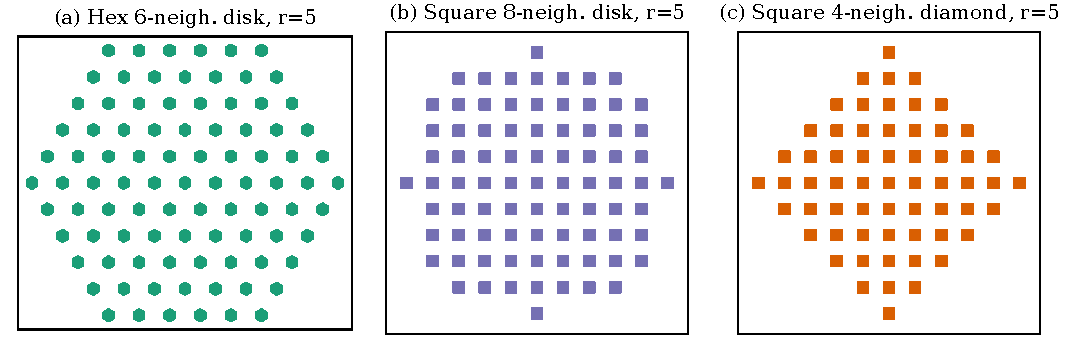
\includegraphics[width=0.98\textwidth]{figures/fig1_method.pdf}
\caption{Filled structuring elements at discrete radius \(r=5\) (physical
half-width \(w=5s\)). (a)~Hexagonal 6-neighborhood disk (91 cells).
(b)~Square 8-neighborhood Euclidean disk (81 cells).
(c)~Square 4-neighborhood diamond (61 cells).}
\label{fig:method}
\end{figure*}

\section{Experimental Design}
\label{sec:exp}

\subsection{Study Windows}
Copernicus GLO-30 is clipped to geographic boxes and warped with
area-weighted averaging from the \(1''\) posting (about \(31\times 25\,\mathrm{m}\)
at these latitudes) to an Albers equal-area 30\,m grid; coarser rasters are
aggregated with the same kernel.
The primary box is loess gully terrain on the Yan River,
\(109.28^\circ\)--\(109.62^\circ\)\,E, \(36.48^\circ\)--\(36.78^\circ\)\,N
(\(998\times 1131\) cells at 30\,m; relief \(496\,\mathrm{m}\); mean slope
\(21^\circ\)).
\rev{The box includes Yan'an and terraces; a northern sub-window
(\(36.65^\circ\)--\(36.78^\circ\)\,N) is used as a spatial split, not as a
second biome.}
The confirmation box is the western margin of the Sichuan basin,
\(103.55^\circ\)--\(103.85^\circ\)\,E, \(30.55^\circ\)--\(30.82^\circ\)\,N
(\(948\times 1012\) cells; relief \(302\,\mathrm{m}\); mean slope \(2.4^\circ\)):
\rev{low-relief, partly settled terrain, not steep humid hills.}
Both are study windows, not hydrographic watersheds.
\rev{At 30\,m the Yan River arm has \(1.05\times 10^6\) valid hexagonal cells
(\(35\%\) of the axial array) versus \(1.13\times 10^6\) valid square cells.}

\subsection{Experiments}
All tests share \(R_{\max}=12\) and the meter axis.
\rev{Decision rules defined a priori in the initial submission are retired:
results are effect sizes.}
\begin{itemize}
\item \textbf{E1} (scale): aggregate to 60, 90, 120\,m, rebuild each tessellation,
compare peak drift, mean drift, and \(W_1\) against the 30\,m spectrum.
\item \textbf{E2} (rotation): lattice protocol on Yan River; DEM protocol for
continuity with the initial submission.
\item \textbf{E3} (neighborhood and SE area): square 4- versus 8-neighborhood,
plus a square radius matched to hexagonal SE area.
\item \textbf{E4} (confirmation; E5 in the initial numbering): full 30--120\,m
protocol on Sichuan and on the Yan River northern split. No separate E4 was
run in the initial submission.
\end{itemize}
\rev{Sensitivity checks: bilinear and nearest-neighbor hex sampling; hexagonal
spacing \(\approx 1.075s\) (equal cell area); nine \(3\times 3\) tiles of the
Yan River 30-to-60\,m pair; half-cell hexagonal offsets as a resampling noise
floor.}
No closing spectrum and no second DEM product are included: openings remove
convexities (ridges, knobs), whereas gully floors would require closings.
The comparison is therefore a bound on tessellation for ridge-scale opening
spectra, not a full granulometric landform inventory.

\section{Results and Discussion}
\label{sec:results}

\begin{table}[t]
\renewcommand{\arraystretch}{1.12}
\caption{Coarsening from 30\,m to \(\{60,90,120\}\)\,m. Entries are means of
the three pairs. Peak and mean are relative drifts against the 30\,m spectrum
(\(\lvert\Delta\rvert/\lambda_{30}\) and \(\lvert\Delta\bar{w}\rvert/\bar{w}_{30}\));
\(W_1\) is in meters on \([s_{\mathrm{coarse}},360\,\mathrm{m}]\). Hexagonal cells
are area-weighted unless noted. All listed spectra have monotone opening volumes.}
\label{tab:results}
\centering
\setlength{\tabcolsep}{3.2pt}
\footnotesize
\begin{tabular}{lcccccc}
\toprule
Window & \multicolumn{2}{c}{Peak} & \multicolumn{2}{c}{Mean} & \multicolumn{2}{c}{\(W_1\) (m)} \\
\cmidrule(lr){2-3}\cmidrule(lr){4-5}\cmidrule(lr){6-7}
 & Hex & Sq & Hex & Sq & Hex & Sq \\
\midrule
Yan River, area & 0.28 & 0.53 & 1.05 & 1.14 & 5.2 & 13.9 \\
Yan River, bilinear & 0.27 & 0.53 & 1.21 & 1.14 & 4.6 & 13.9 \\
Yan north split, area & 0.11 & 0.53 & 1.02 & 1.12 & 5.0 & 14.1 \\
Sichuan basin margin, area & 2.00 & 0.22 & 1.83 & 1.81 & 4.7 & 13.8 \\
\bottomrule
\end{tabular}
\end{table}

\begin{figure*}[t]
\centering
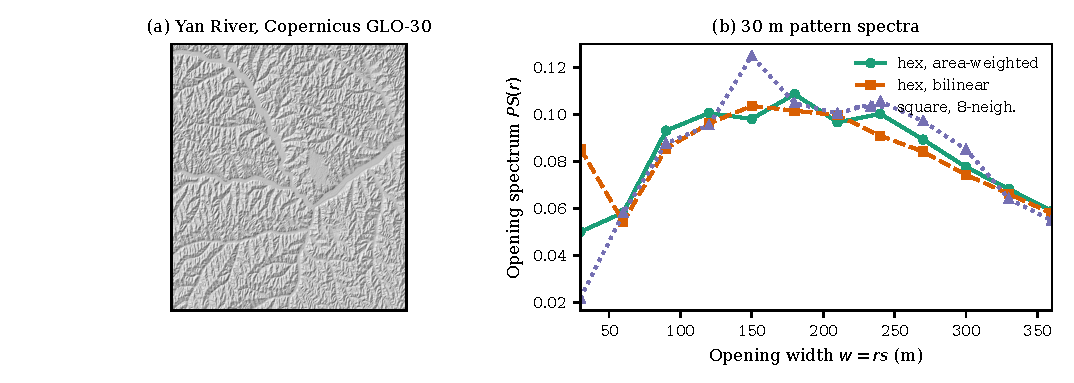
\includegraphics[width=0.98\textwidth]{figures/fig2_dem_spectrum.pdf}
\caption{Primary study box. (a)~Hillshade of Copernicus GLO-30 on the Yan River
loess window (Albers, 30\,m). (b)~Normalized opening spectra. Area-weighted
hexagonal cells peak at \(180\,\mathrm{m}\); bilinear hexagons and the square
8-neighborhood peak at \(150\,\mathrm{m}\).}
\label{fig:dem}
\end{figure*}

Table~\ref{tab:results} collects coarsening effect sizes.
Fig.~\ref{fig:dem} shows the Yan River hillshade and the 30\,m spectra.
\rev{Area-weighted hexagons peak at \(180\,\mathrm{m}\); bilinear hexagons and
square 8-neighborhood disks peak at \(150\,\mathrm{m}\). Switching the hexagonal
estimator therefore moves the discrete peak by one bin already at 30\,m.}

\subsection{Scale Experiment}
On the Yan River, mean relative \emph{peak} drift is 0.28 (area hex) versus 0.53
(square) [Fig.~\ref{fig:scale}(a)].
\rev{The hexagonal sequence is \(180,180,90,240\,\mathrm{m}\); the square sequence
is \(150,180,270,240\,\mathrm{m}\). At 90\,m the hexagonal peak sits on the
Nyquist line \(\lambda=s\), so peak drift is not a landform width.}
The spectral mean [Fig.~\ref{fig:scale}(b)] increases with \(s\) on both lattices
(\(195\to 513\,\mathrm{m}\) hex versus \(200\to 538\,\mathrm{m}\) square); relative
mean drift is 1.05 versus 1.14.
\rev{Common-support \(W_1\) is \(5.2\,\mathrm{m}\) versus \(13.9\,\mathrm{m}\).
That gap survives bilinear sampling (\(4.6\) versus \(13.9\)), equal-area hexagonal
spacing \(1.075s\) (\(5.0\) versus \(13.9\)), and a square radius matched to
hexagonal SE area at each \(r\) (square \(W_1=24.4\,\mathrm{m}\) on the 30-to-120\,m
pair versus hexagonal \(5.8\,\mathrm{m}\)).
Nearest-neighbor hex sampling inflates 30-to-120\,m \(W_1\) to \(9.3\,\mathrm{m}\).
Nine tiles of the 30-to-60\,m pair give median mean-drift \(0.48\) (IQR \(0.12\))
hexagonal versus \(0.60\) (\(0.06\)) square; median \emph{peak} drift reverses
(\(0.67\) versus \(0.20\)); median \(W_1\) is \(9.7\,\mathrm{m}\) (IQR \(6.9\,\mathrm{m}\))
versus \(10.8\,\mathrm{m}\) (\(0.6\,\mathrm{m}\)). Half-cell hexagonal offsets yield a
bilinear \(W_1\) floor of \(0.14\)--\(0.29\,\mathrm{m}\), well below the
whole-window coarsening \(W_1\), but an area-weighted \(q\)-shift reaches
\(8.1\,\mathrm{m}\), comparable to the headline hexagonal \(W_1\) of \(5.2\,\mathrm{m}\).
Lattice phase of pixel-to-hex binning is therefore a confound, and the
hexagonal \(W_1\) advantage is not a tight tile-level effect.}

\begin{figure*}[t]
\centering
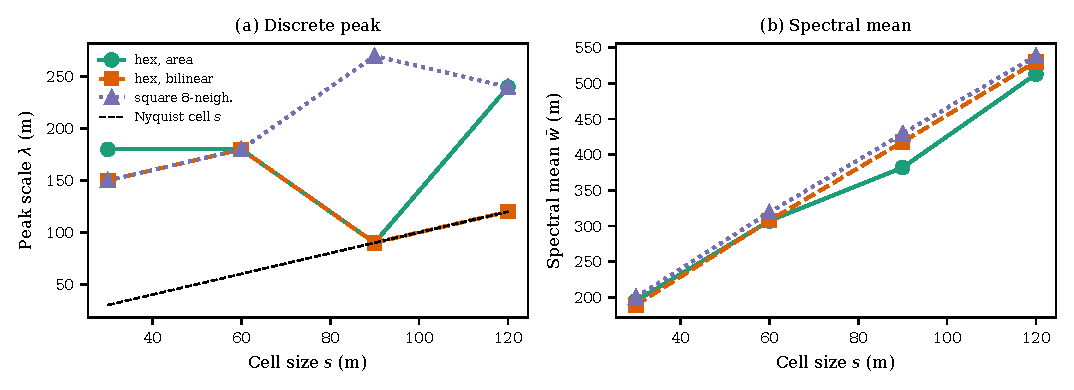
\includegraphics[width=0.98\textwidth]{figures/fig3_scale.pdf}
\caption{Scale experiment on the Yan River box. (a)~Discrete peak versus cell
size, with the Nyquist bound \(\lambda=s\). (b)~Spectral mean \(\bar{w}\).}
\label{fig:scale}
\end{figure*}

\subsection{Rotation Experiment}
\rev{Lattice rotation with bilinear hex sampling gives maximum \(W_1\) of
\(2.58\,\mathrm{m}\) (hex, \(60^\circ\)) versus \(2.62\,\mathrm{m}\) (square,
\(45^\circ\)): a near-tie, with hexagons worse at \(60^\circ\) on windowed \(L^1\)
(\(0.031\) versus \(0.027\)).
Area-weighted lattice rotation \emph{increases} hexagonal \(W_1\) to
\(4.0\)--\(5.5\,\mathrm{m}\) because rotating the hex bins reassigns square pixels
[Fig.~\ref{fig:rot}(a)].
DEM rotation of the bilinear protocol reproduces the initial submission:
windowed \(L^1\) maxima \(0.033\) (hex) versus \(0.030\) (square)
[Fig.~\ref{fig:rot}(b)].
A Euclidean disk on the square grid is already nearly circular for \(r\gtrsim 3\),
whereas a hexagon has circumradius-to-inradius ratio \(2/\sqrt{3}\approx 1.155\)
at every \(r\); a hexagonal rotational advantage is therefore not guaranteed.}

\begin{figure*}[t]
\centering
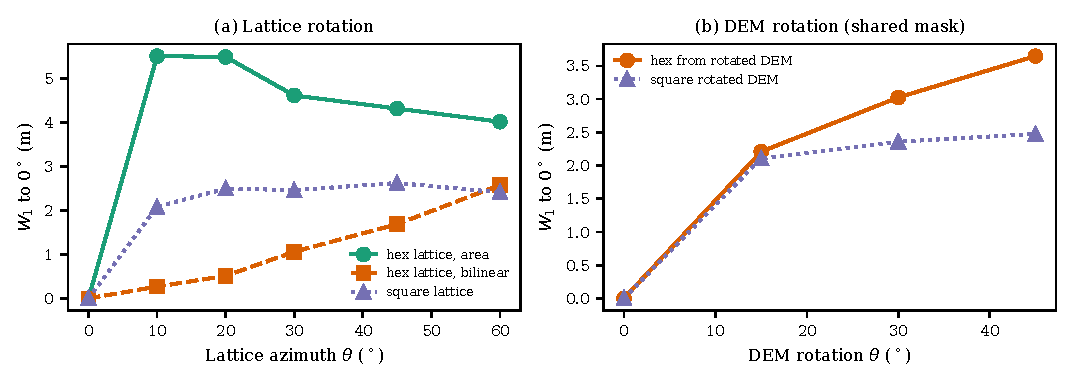
\includegraphics[width=0.98\textwidth]{figures/fig4_rotation.pdf}
\caption{Rotational \(W_1\) to \(0^\circ\) on the Yan River box.
(a)~Lattice rotation on an interior mask.
(b)~DEM rotation with a shared valid mask.}
\label{fig:rot}
\end{figure*}

\subsection{Neighborhood Experiment}
For 30-to-60\,m on Yan River, full-axis \(L^1\) remains
\(0.728\) (hex), \(0.708\) (square-8), \(0.741\) (square-4): hexagons sit between
the two square operators.
\rev{On common-support \(W_1\) the ranking does not flip:
\(2.0\,\mathrm{m}\) (hex), \(11.2\,\mathrm{m}\) (square-8), \(6.0\,\mathrm{m}\)
(square-4). Sichuan \(W_1\) is \(2.1\), \(12.7\), and \(7.8\,\mathrm{m}\).
The 4-neighborhood diamond is the Minkowski generator comparable to the hex
disk; the 8-neighborhood Euclidean disk is the more circular square operator
used in remote-sensing morphological profiles. Both are required as controls.}

\subsection{Confirmation Experiment}
On the Sichuan basin-margin window the 30\,m hexagonal peak is already at one
cell (\(30\,\mathrm{m}\)) while the square peak is at \(90\,\mathrm{m}\).
Running the same three coarsening steps as E1, mean peak drift is 2.00 versus 0.22
and the hexagonal peak remains on the Nyquist line at every \(s\).
Spectral-mean drift is tied (\(1.83\) versus \(1.81\)).
\rev{\(W_1\) still favors hexagons (\(4.7\) versus \(13.8\,\mathrm{m}\)).
The northern Yan River split tracks the parent loess box (peak \(0.11\) versus
\(0.53\); \(W_1\) \(5.0\) versus \(14.1\,\mathrm{m}\)).
Two landscapes plus one spatial split do not represent a biome: the peak ranking
is landscape-dependent; the common-support \(W_1\) ranking is not, in this set.}

Taken together, the result that survives isolation checks on dissected loess is
a \emph{conditional} reduction of coarsening-induced spectral transport (\(W_1\)),
not a stable peak landform width and not a rotational upgrade.
A claim that hexagonal morphological spectra are generally more stable would
overstate the evidence.
\rev{Practically, a downstream user who selects a morphological-profile scale from
the discrete peak would not obtain a reliable hexagonal benefit, especially on
low-relief DSM terrain where the peak hugs Nyquist.
A user who treats the meter-aligned spectrum as a descriptor (for example a
feature for morphological profiles~\cite{pesaresi2001new}) would see a smaller
\(W_1\) under coarsening on these windows, of order \(5\,\mathrm{m}\) versus
\(14\,\mathrm{m}\) on a \(30\)--\(360\,\mathrm{m}\) support, above the bilinear
offset floor but comparable to area-weighted lattice-phase noise
(\(8.1\,\mathrm{m}\)) and not recovered as a small tile IQR.}

Limitations follow from the design. Openings, not closings. \(R_{\max}=12\)
truncates gully-scale mass wider than \(360\,\mathrm{m}\).
GLO-30 is a DSM~\cite{guth2021lidar,simard2024global}.
The lattice is local Albers, not ISEA.
Area-weighted hexagons still live on an underlying square posting.
Two windows cannot represent a landform class.

\section{Conclusion}

\rev{On Yan River loess, whole-window hexagonal opening spectra change less under
30-to-120\,m coarsening than square 8-neighborhood spectra when change is
measured by common-support \(W_1\) (\(\approx 5\,\mathrm{m}\) versus
\(14\,\mathrm{m}\)).
Bilinear sampling, SE-area mismatch, and unequal cell area do not create that
whole-window gap, but area-weighted lattice-phase noise (\(8.1\,\mathrm{m}\))
is of the same order, and nine-tile 30-to-60\,m \(W_1\) is only \(9.7\,\mathrm{m}\)
versus \(10.8\,\mathrm{m}\) with a large hexagonal IQR.
The discrete peak is a poor proxy: it favors hexagons on loess, reverses on
Sichuan, and reverses across tiles.
Rotational \(W_1\) is a near-tie under bilinear lattice sampling and worse for
area-weighted hexagons.
Hexagonal tessellation is therefore a useful control in DEM morphology---not a
drop-in isotropic upgrade, and not a large practical margin on these windows.}

\section*{Acknowledgment}

Copernicus GLO-30 \(\copyright\) DLR e.V.\ 2010--2014 and \(\copyright\)
Airbus Defence and Space GmbH 2014--2018, provided under Copernicus by
the European Union and ESA.
\rev{Python code, window definitions, and tabulated spectra that reproduce the
experiments are at
\url{https://github.com/fariell/Scale-Stability-of-Terrain-Opening-Spectra-on-Hexagonal-Versus-Square-Grids}
and as journal supplementary files.}
The author conceived the study, performed the experiments, and wrote the
manuscript. The author declares no conflicts of interest.

\bibliographystyle{IEEEtran}
\bibliography{refs}

\end{document}
